%******************************************************************************%
%                                                                              %
%                  sample.en.tex for LaTeX                                     %
%                  Created on : Tue Mar 10 13:27:28 2015                       %
%                  Made by : David "Thor" GIRON <thor@42.fr>                   %
%                                                                              %
%******************************************************************************%

\documentclass{42-en}


%******************************************************************************%
%                                                                              %
%                                    Header                                    %
%                                                                              %
%******************************************************************************%
\begin{document}



                           \title{Structured Query Language: Basics!}
                          \subtitle{The world is a zoo, you've seen the news}
                       \member{Ted Tran}{ttran@student.42.us.org}
                        \member{42 Ghost Bum}{pedago@42.fr}

\summary {
  This project is an introduction to \texttt{SQL} using material 
  from \href{https://sqlzoo.net}{SQLZoo}.
}

\maketitle

\tableofcontents


%******************************************************************************%
%                                                                              %
%                                  Foreword                                    %
%                                                                              %
%******************************************************************************%
\chapter{Foreword}

	You know, at the end of the day, if you're stuck, you can easily get the 
	vast majority of answers using google. SQLBolt and SQLZoo are probably 
	the most popular resources to learn SQL these days. \\
	
	But have no fear! \\ 

	I wrote a \texttt{TON} of extra queries for you all to complete and have fun 
	doing. And by fun, I mean as fun as falling into a gorilla closure at a 
	zoo. Prepare for a world of \texttt{hurt} due to one man's good intentions. \\

	Good luck! \\

	If you need help, you won't get it until you go onto the HackHighSchool slack 
	and @(any mentor who's not in charge of the SQL curriculum) 10 times and show me proof. \\

	And remember-- please try solving the problem on your own using your massive brain, 
	Google, or asking your peers before coming to me. \\ 

	I'm sure you're wondering, "Why is this foreword so long?". I'll tell you why, the real truth. 
	It's because the xkcd comic on the page after this one is so long, so I need to put filler 
	text in to fill this page so it doesn't look empty. \\

	You know what? I think you're being ungrateful. Just because of that, I'm going to write 
	the rest of the learning material in French then google translate it into Vietnamese, 
	Spanish, Japanese, and German before English to get the real authenticity of a 42 PDF. \\ 

	But have no fear, High School students! -> Do not worry, student!

    % Spacing in the source code does not influence spacing in the
    % generated pdf. The blank lines aboves and below won't appear.
    % Instead, use \newline (or its shortcut \\) and \newpage to
    % create vertical spacing.
    
            \begin{figure}[H]
                \begin{center}
                    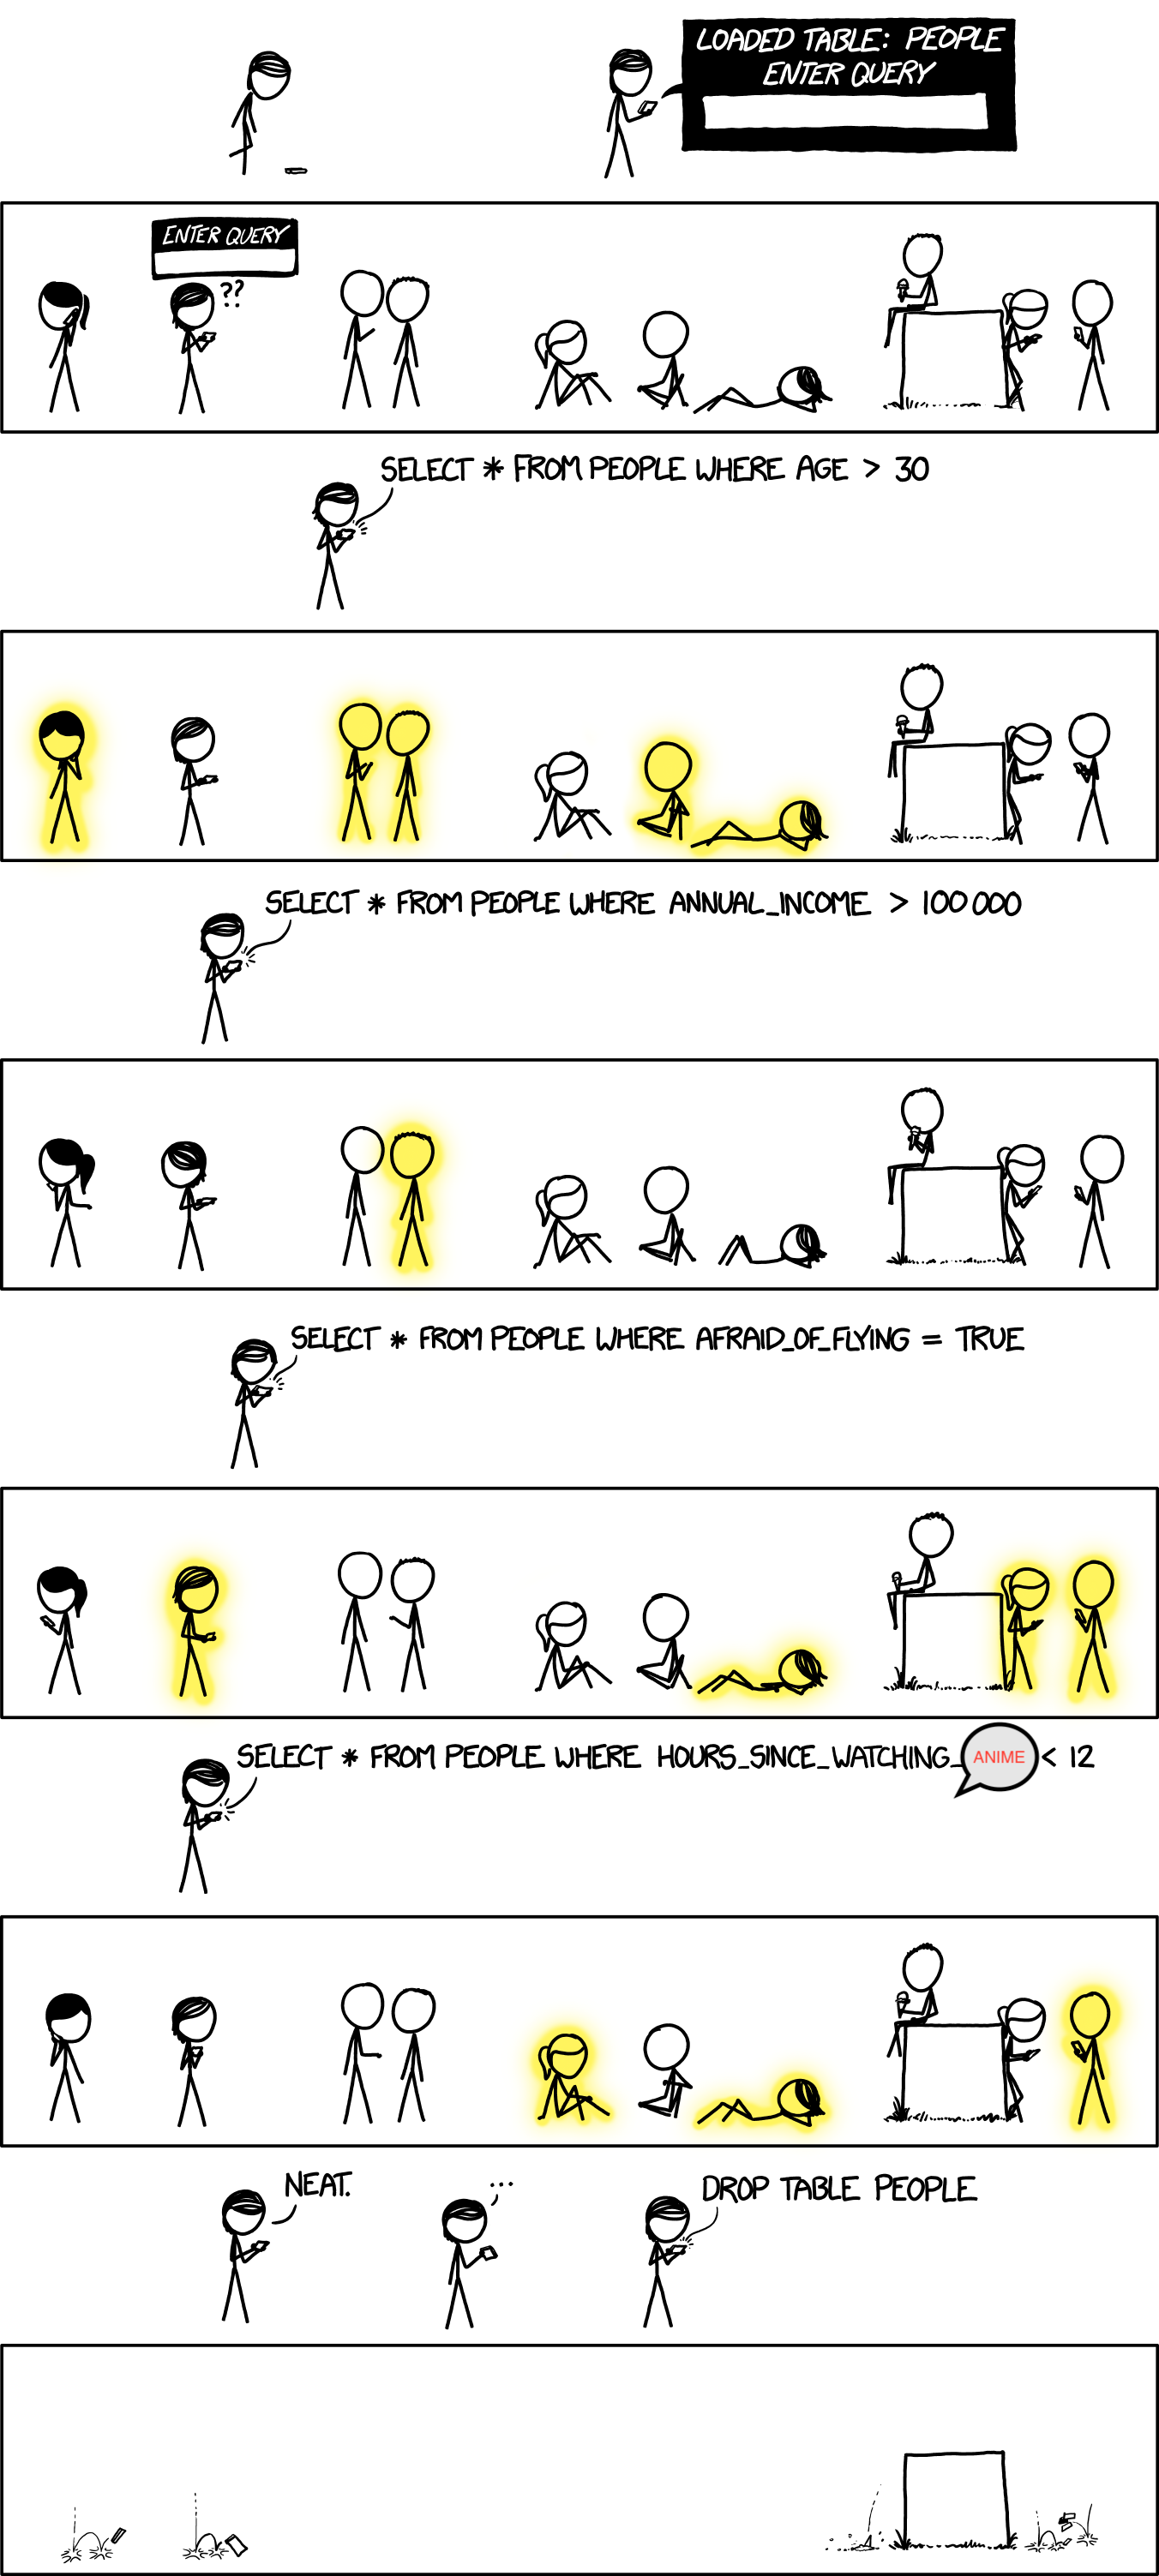
\includegraphics[width=10cm]{query_2x.png}
                \end{center}
            \end{figure}

	    	\newpage 	

%******************************************************************************%
%                                                                              %
%                                 Introduction                                 %
%                                                                              %
%******************************************************************************%
\chapter{Introduction}

	What the hell am I going to be doing?

	\begin{itemize}\itemsep1pt
		\item First, you're going to be running a ton of docker commands 
			so that you can run various things on these 42 lab computers
		\item Next, you're going to be learning all the SQL fundamentals! 
		\item It'll be learning through experience, so be prepared to write 
			a ridiculous amount of queries. 
		\item Once you have the fundamentals down, it'll be time for you to 
			write a wrapper so users can interact with the database 
			without writing any SQL queries(since you wrote em' already!) 
	\end{itemize}


%******************************************************************************%
%                                                                              %
%                                  Goals                                       %
%                                                                              %
%******************************************************************************%
\chapter{Goals}

    This chapter introduces the pedagogical interests of your project,
    because in the end, a project is only a mean to explore and
    discover new topics. For instance our \texttt{42} \texttt{C++}
    project \texttt{Nibbler}. Despite being just a simple
    \texttt{Snake} game, this project introduces the students to the
    creation of an API and some plugins for a \texttt{C++} program.


%******************************************************************************%
%                                                                              %
%                             General instructions                             %
%                                                                              %
%******************************************************************************%
\chapter{General instructions}

    This chapter lists all basic instructions of a project.
    Language, restrictions, permissions, compilation, etc.


% Don't forget this line for piscine days to initate the exercise counter at 0
\startexercices

%******************************************************************************%
%                                                                              %
%                             Day of the Piscine                               %
%                                                                              %
%******************************************************************************%

\chapter{Exercise \exercicenumber: A Day of the Piscine}

\extitle{Title}
\exnumber{\exercicenumber}
\exfiles{expected\_file.py}
\exforbidden{Forbidden functions}
\exnotes{Notes}

\makeheaderfiles

    This is an example of how to format the headings on a piscine-style multi part
    challenge.

% Don't forget this line in order to increment the exercise counter
\nextexercice

%******************************************************************************%
%                                                                              %
%                             Mandatory part                                   %
%                                                                              %
%******************************************************************************%
\chapter{Mandatory part}

    Heart of the subject, the mandatory part describes in details the
    work expected and the possible tools and/or technologies
    required. The secret of a good subject is the balance between
    being specific and leaving a part to the interpretation and
    imagination. This balance is very important as it is the engine
    that fuels debates and argumentations during peer-evaluation.



%******************************************************************************%
%                                                                              %
%                                 Bonus part                                   %
%                                                                              %
%******************************************************************************%
\chapter{Bonus part}

    When a student invests time in a project and the goals are met,
    it's innate to will to go further ! The bonus section is here to satisfy
    such ambition. Of course, the bonus part is exclusively available
    if and only if the mandatory part is complete and perfect.



%******************************************************************************%
%                                                                              %
%                           Turn-in and peer-evaluation                        %
%                                                                              %
%******************************************************************************%
\chapter{Turn-in and peer-evaluation}

    This part describes the conditions and instructions regarding the turn-in and
    the peer-evaluation of the project. If your project does not
    require odd turn-in or peer-evaluation instructions, feel free to
    use the following paragraph as it is:\\

    Turn your work in using your \texttt{GiT} repository, as
    usual. Only work present on your repository will be graded in defense.



%******************************************************************************%
\end{document}
